

\tikzset{every picture/.style={line width=0.75pt}} %set default line width to 0.75pt        

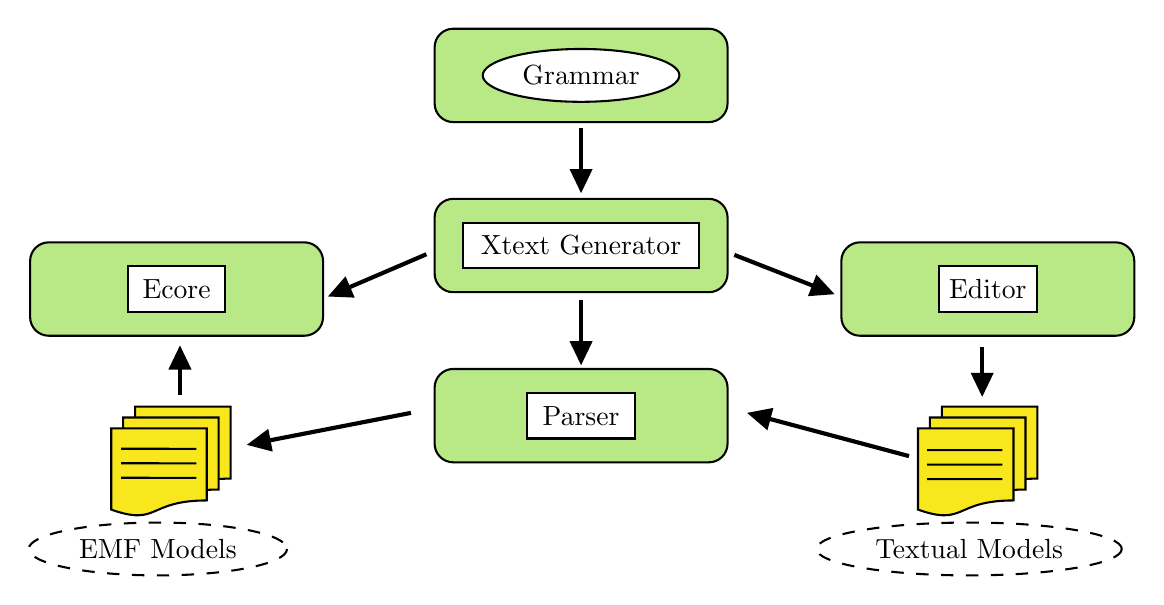
\begin{tikzpicture}[x=0.75pt,y=0.75pt,yscale=-1,xscale=1]
%uncomment if require: \path (0,440.1999969482422); %set diagram left start at 0, and has height of 440.1999969482422

%Rounded Rect [id:dp8080613887465731] 
\draw  [fill={rgb, 255:red, 184; green, 233; blue, 134 }  ,fill opacity=1 ] (268.19,31.77) .. controls (268.19,26.8) and (272.21,22.77) .. (277.18,22.77) -- (400.33,22.77) .. controls (405.3,22.77) and (409.33,26.8) .. (409.33,31.77) -- (409.33,58.76) .. controls (409.33,63.73) and (405.3,67.76) .. (400.33,67.76) -- (277.18,67.76) .. controls (272.21,67.76) and (268.19,63.73) .. (268.19,58.76) -- cycle ;

%Rounded Rect [id:dp23877247410758984] 
\draw  [fill={rgb, 255:red, 184; green, 233; blue, 134 }  ,fill opacity=1 ] (464.16,134.7) .. controls (464.16,129.73) and (468.19,125.7) .. (473.15,125.7) -- (596.3,125.7) .. controls (601.27,125.7) and (605.3,129.73) .. (605.3,134.7) -- (605.3,161.69) .. controls (605.3,166.66) and (601.27,170.69) .. (596.3,170.69) -- (473.15,170.69) .. controls (468.19,170.69) and (464.16,166.66) .. (464.16,161.69) -- cycle ;

%Rounded Rect [id:dp8660361288400333] 
\draw  [fill={rgb, 255:red, 184; green, 233; blue, 134 }  ,fill opacity=1 ] (268.19,113.73) .. controls (268.19,108.76) and (272.21,104.74) .. (277.18,104.74) -- (400.33,104.74) .. controls (405.3,104.74) and (409.33,108.76) .. (409.33,113.73) -- (409.33,140.72) .. controls (409.33,145.69) and (405.3,149.72) .. (400.33,149.72) -- (277.18,149.72) .. controls (272.21,149.72) and (268.19,145.69) .. (268.19,140.72) -- cycle ;

%Rounded Rect [id:dp8159423215616721] 
\draw  [fill={rgb, 255:red, 184; green, 233; blue, 134 }  ,fill opacity=1 ] (73.3,134.7) .. controls (73.3,129.73) and (77.33,125.7) .. (82.3,125.7) -- (205.45,125.7) .. controls (210.41,125.7) and (214.44,129.73) .. (214.44,134.7) -- (214.44,161.69) .. controls (214.44,166.66) and (210.41,170.69) .. (205.45,170.69) -- (82.3,170.69) .. controls (77.33,170.69) and (73.3,166.66) .. (73.3,161.69) -- cycle ;

%Rounded Rect [id:dp9641259565957541] 
\draw  [fill={rgb, 255:red, 184; green, 233; blue, 134 }  ,fill opacity=1 ] (268.19,195.7) .. controls (268.19,190.73) and (272.21,186.7) .. (277.18,186.7) -- (400.33,186.7) .. controls (405.3,186.7) and (409.33,190.73) .. (409.33,195.7) -- (409.33,222.69) .. controls (409.33,227.66) and (405.3,231.68) .. (400.33,231.68) -- (277.18,231.68) .. controls (272.21,231.68) and (268.19,227.66) .. (268.19,222.69) -- cycle ;

%Flowchart: Multidocument [id:dp814245162277164] 
\draw  [fill={rgb, 255:red, 248; green, 231; blue, 28 }  ,fill opacity=1 ] (123.89,204.81) -- (169.93,204.81) -- (169.93,239.53) .. controls (141.16,239.53) and (146.91,252.05) .. (123.89,243.95) -- cycle ; \draw  [fill={rgb, 255:red, 248; green, 231; blue, 28 }  ,fill opacity=1 ] (118.14,210.07) -- (164.17,210.07) -- (164.17,244.79) .. controls (135.4,244.79) and (141.16,257.31) .. (118.14,249.21) -- cycle ; \draw  [fill={rgb, 255:red, 248; green, 231; blue, 28 }  ,fill opacity=1 ] (112.39,215.33) -- (158.42,215.33) -- (158.42,250.05) .. controls (129.65,250.05) and (135.4,262.57) .. (112.39,254.47) -- cycle ;
%Straight Lines [id:da659202853659377] 
\draw    (117.13,225.14) -- (153.43,225.17) ;


%Straight Lines [id:da8271632436642871] 
\draw    (117.13,232.13) -- (153.43,232.16) ;


%Straight Lines [id:da22701123408508272] 
\draw    (117.13,239.12) -- (153.43,239.15) ;




%Flowchart: Multidocument [id:dp49717070559395604] 
\draw  [fill={rgb, 255:red, 248; green, 231; blue, 28 }  ,fill opacity=1 ] (512.58,204.81) -- (558.61,204.81) -- (558.61,239.53) .. controls (529.84,239.53) and (535.6,252.05) .. (512.58,243.95) -- cycle ; \draw  [fill={rgb, 255:red, 248; green, 231; blue, 28 }  ,fill opacity=1 ] (506.83,210.07) -- (552.86,210.07) -- (552.86,244.79) .. controls (524.09,244.79) and (529.84,257.31) .. (506.83,249.21) -- cycle ; \draw  [fill={rgb, 255:red, 248; green, 231; blue, 28 }  ,fill opacity=1 ] (501.07,215.33) -- (547.11,215.33) -- (547.11,250.05) .. controls (518.33,250.05) and (524.09,262.57) .. (501.07,254.47) -- cycle ;
%Straight Lines [id:da5642847406466045] 
\draw [fill={rgb, 255:red, 248; green, 231; blue, 28 }  ,fill opacity=1 ]   (505.45,225.77) -- (541.75,225.81) ;


%Straight Lines [id:da9779186616916171] 
\draw [fill={rgb, 255:red, 248; green, 231; blue, 28 }  ,fill opacity=1 ]   (505.45,232.76) -- (541.75,232.8) ;


%Straight Lines [id:da8217185402464098] 
\draw [fill={rgb, 255:red, 248; green, 231; blue, 28 }  ,fill opacity=1 ]   (505.45,239.75) -- (541.75,239.78) ;




%Straight Lines [id:da4555835119587406] 
\draw [line width=1.5]    (338.76,70.52) -- (338.76,98.97) ;
\draw [shift={(338.76,101.97)}, rotate = 270] [fill={rgb, 255:red, 0; green, 0; blue, 0 }  ][line width=1.5]  [draw opacity=0] (11.61,-5.58) -- (0,0) -- (11.61,5.58) -- cycle    ;

%Straight Lines [id:da2586670416419199] 
\draw [line width=1.5]    (338.76,153.44) -- (338.76,181.89) ;
\draw [shift={(338.76,184.89)}, rotate = 270] [fill={rgb, 255:red, 0; green, 0; blue, 0 }  ][line width=1.5]  [draw opacity=0] (11.61,-5.58) -- (0,0) -- (11.61,5.58) -- cycle    ;

%Straight Lines [id:da2552674310073062] 
\draw [line width=1.5]    (264.22,131.44) -- (219.57,150.59) ;
\draw [shift={(216.81,151.77)}, rotate = 336.78999999999996] [fill={rgb, 255:red, 0; green, 0; blue, 0 }  ][line width=1.5]  [draw opacity=0] (11.61,-5.58) -- (0,0) -- (11.61,5.58) -- cycle    ;

%Straight Lines [id:da29550662771480396] 
\draw [line width=1.5]    (458.11,149.58) -- (412.6,131.75) ;

\draw [shift={(460.9,150.67)}, rotate = 201.39] [fill={rgb, 255:red, 0; green, 0; blue, 0 }  ][line width=1.5]  [draw opacity=0] (11.61,-5.58) -- (0,0) -- (11.61,5.58) -- cycle    ;
%Straight Lines [id:da3813677861719633] 
\draw [line width=1.5]    (532.01,176.31) -- (532.01,197.14) ;
\draw [shift={(532.01,200.14)}, rotate = 270] [fill={rgb, 255:red, 0; green, 0; blue, 0 }  ][line width=1.5]  [draw opacity=0] (11.61,-5.58) -- (0,0) -- (11.61,5.58) -- cycle    ;

%Straight Lines [id:da3940907258410822] 
\draw [line width=1.5]    (145.5,178.36) -- (145.5,199.18) ;

\draw [shift={(145.5,175.36)}, rotate = 90] [fill={rgb, 255:red, 0; green, 0; blue, 0 }  ][line width=1.5]  [draw opacity=0] (11.61,-5.58) -- (0,0) -- (11.61,5.58) -- cycle    ;
%Straight Lines [id:da3280771928101003] 
\draw [line width=1.5]    (256.79,207.86) -- (180.67,222.68) ;
\draw [shift={(177.73,223.25)}, rotate = 348.98] [fill={rgb, 255:red, 0; green, 0; blue, 0 }  ][line width=1.5]  [draw opacity=0] (11.61,-5.58) -- (0,0) -- (11.61,5.58) -- cycle    ;

%Straight Lines [id:da9478402467031726] 
\draw [line width=1.5]    (496.73,228.68) -- (421.65,208.63) ;
\draw [shift={(418.76,207.86)}, rotate = 374.95] [fill={rgb, 255:red, 0; green, 0; blue, 0 }  ][line width=1.5]  [draw opacity=0] (11.61,-5.58) -- (0,0) -- (11.61,5.58) -- cycle    ;


% Text Node
\draw  [fill={rgb, 255:red, 255; green, 255; blue, 255 }  ,fill opacity=1 ]  (511.23,137.2) -- (558.23,137.2) -- (558.23,159.2) -- (511.23,159.2) -- cycle  ;
\draw (534.73,148.2) node  [align=left] {Editor};
% Text Node
\draw  [fill={rgb, 255:red, 255; green, 255; blue, 255 }  ,fill opacity=1 ]  (120.37,137.2) -- (167.37,137.2) -- (167.37,159.2) -- (120.37,159.2) -- cycle  ;
\draw (143.87,148.2) node  [align=left] {Ecore};
% Text Node
\draw  [fill={rgb, 255:red, 255; green, 255; blue, 255 }  ,fill opacity=1 ]  (312.76,198.19) -- (364.76,198.19) -- (364.76,220.19) -- (312.76,220.19) -- cycle  ;
\draw (338.76,209.19) node  [align=left] {Parser};
% Text Node
\draw  [dash pattern={on 4.5pt off 4.5pt}]  (134.86, 273.43) circle [x radius= 62.23, y radius= 12.73]   ;
\draw (134.86,273.43) node  [align=left] {EMF Models};
% Text Node
\draw  [dash pattern={on 4.5pt off 4.5pt}]  (525.72, 273.43) circle [x radius= 73.54, y radius= 12.73]   ;
\draw (525.72,273.43) node  [align=left] {Textual Models};
% Text Node
\draw  [fill={rgb, 255:red, 255; green, 255; blue, 255 }  ,fill opacity=1 ]  (338.76, 45.26) circle [x radius= 47.38, y radius= 12.73]   ;
\draw (338.76,45.26) node  [align=left] {Grammar};
% Text Node
\draw  [fill={rgb, 255:red, 255; green, 255; blue, 255 }  ,fill opacity=1 ]  (281.76,116.23) -- (395.76,116.23) -- (395.76,138.23) -- (281.76,138.23) -- cycle  ;
\draw (338.76,127.23) node  [align=left] {Xtext Generator};


\end{tikzpicture}
